\section{センサノードグループ化のアプローチ}

% --- トポロジ ---
\subsection{トポロジ}
グループは,ある数のセンサノードから構成される.グループのトポロジは,グループ内での通信とGLノードとGWノードの通信と2種類ある.ノード間通信は,前者にBLE,後者にLoRaWANを用いる.

\begin{figure}[]
    \begin{center}
    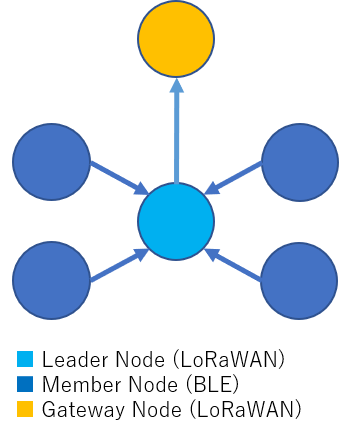
\includegraphics[width=5cm]{figures/グループ化のトポロジ.png}
    \caption{グループ化のトポロジ}
    \label{fig:group_topology}
    \end{center}
\end{figure}

% --- センサネットワーク展開時のグループ化 ---
\subsection{センサネットワーク展開時のグループ化}
センサネットワークが展開される初回起動時にグループを作成する手法を述べる.GWノードがセンサノードのトポロジを把握するため,各ノードが周囲のノード情報を探索する.下記にシーケンス図\ref{fig:group_on_activation}を示す.

\begin{enumerate}
    \item グループを構築するに当たり,GWノードに現在のWSNトポロジを通知する必要がある.そのため,センサノード起動時に,BLEにて自身の情報を発信し,同時に周囲のセンサノード情報を収集する.近傍センサノードのリストを作成した後,GWノードへ送信する.
    \item センサノードはリスト送信後,GWノードからグループ構成の通知が来るまでLoRaWANにて通信を行う.
    \item GWノードがセンサノード情報を集約した後,センサノードの固有ID,及び個々の信号強度を用いて重複ノードのないグループを作成しグループごとに1つGLノードを選出する.センサノードがLoRaWANにて次に接続した場合,Downlinkでグループ構成を通知しシーケンスは終了する.
\end{enumerate}

\begin{figure}[]
    \begin{center}
    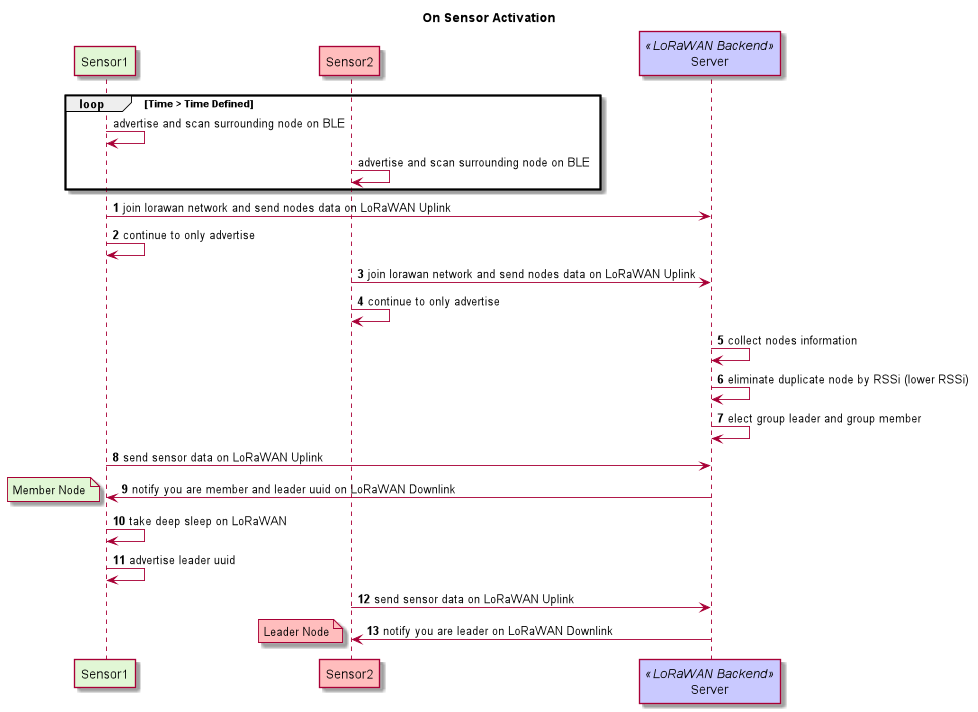
\includegraphics[width=14cm]{figures/グループ化_センサ起動時.png}
    \caption{グループ化の通信方式}
    \label{fig:group_on_activation}
    \end{center}
\end{figure}

% --- 平常時のグループ化の通信 ---
\subsection{平常時のグループ化の通信}
平常時のグループの通信フローを述べる.通信方式は,グループ内の通信にBLE,GLノードとGWノードの通信にLoRaWANを用いる.グループ内の通信は,インターバルが設けられ同期的に通信を行う.下記にシーケンス図\ref{fig:default_data_flow}を示す.

\begin{enumerate}
    \item GMノードはGLノードとの接続要求のため,Advを開始する.
    \item GLノードはGMノードとの接続確立のため,BLEにてScanを開始する.
    \item GLノードは接続確立後,GMノードからセンサデータを集約しGWへ送信する.
    \item WSNに新たなノードが参加した際にグループに所属するため,GLは自身のサービスUUIDを載せAdvを開始する.
\end{enumerate}

\begin{figure}[]
    \begin{center}
    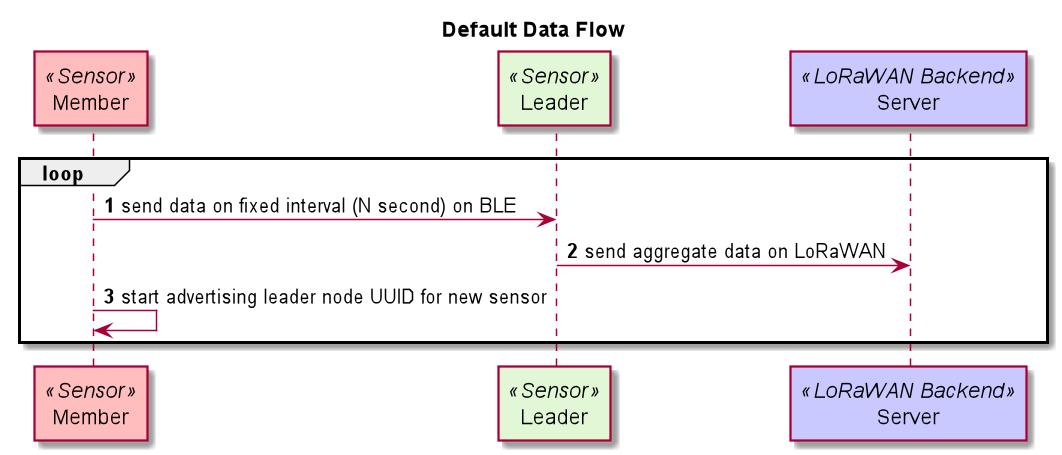
\includegraphics[width=13cm]{figures/グループ化の通信方式.png}
    \caption{グループ化の通信方式}
    \label{fig:default_data_flow}
    \end{center}
\end{figure}

% --- センサノードの参加・離脱時の振る舞い ---
\subsection{センサノードの参加・離脱時の振る舞い}
いくつかのセンサノードが,グループへ参加・離脱する際の手法を述べる.\\ \\
前者について下記にシーケンス図\ref{fig:group_on_join}を示す.

\begin{enumerate}
    \item 新規センサノードがグループに参加するため,参加するグループを決定する必要がある.GLノードはデータ集約時以外は,Adv Packetに自身のBLEサービスUUIDを載せAdvを行う.
    \item 新規センサノードは,起動時にBLEスキャンを実行し周囲に参加可能なグループがあるか探索する.
    \item 発見した場合は,そのグループに参加し,そうでない場合はLoRaWANで直接センサデータを送信する.
\end{enumerate}

後者について,下記にシーケンス図\ref{fig:group_on_leave}を示す.

\begin{enumerate}
    \item ノードが故障や電池切れで離脱する場合は,NSがデバイスを管理しているので,N回通信が来なかった場合に,グループリストからセンサノードを取り除く.
    \item GLノードの次回通信時に,更新したグループリストを通知する.
\end{enumerate}

\begin{figure}[]
    \begin{center}
    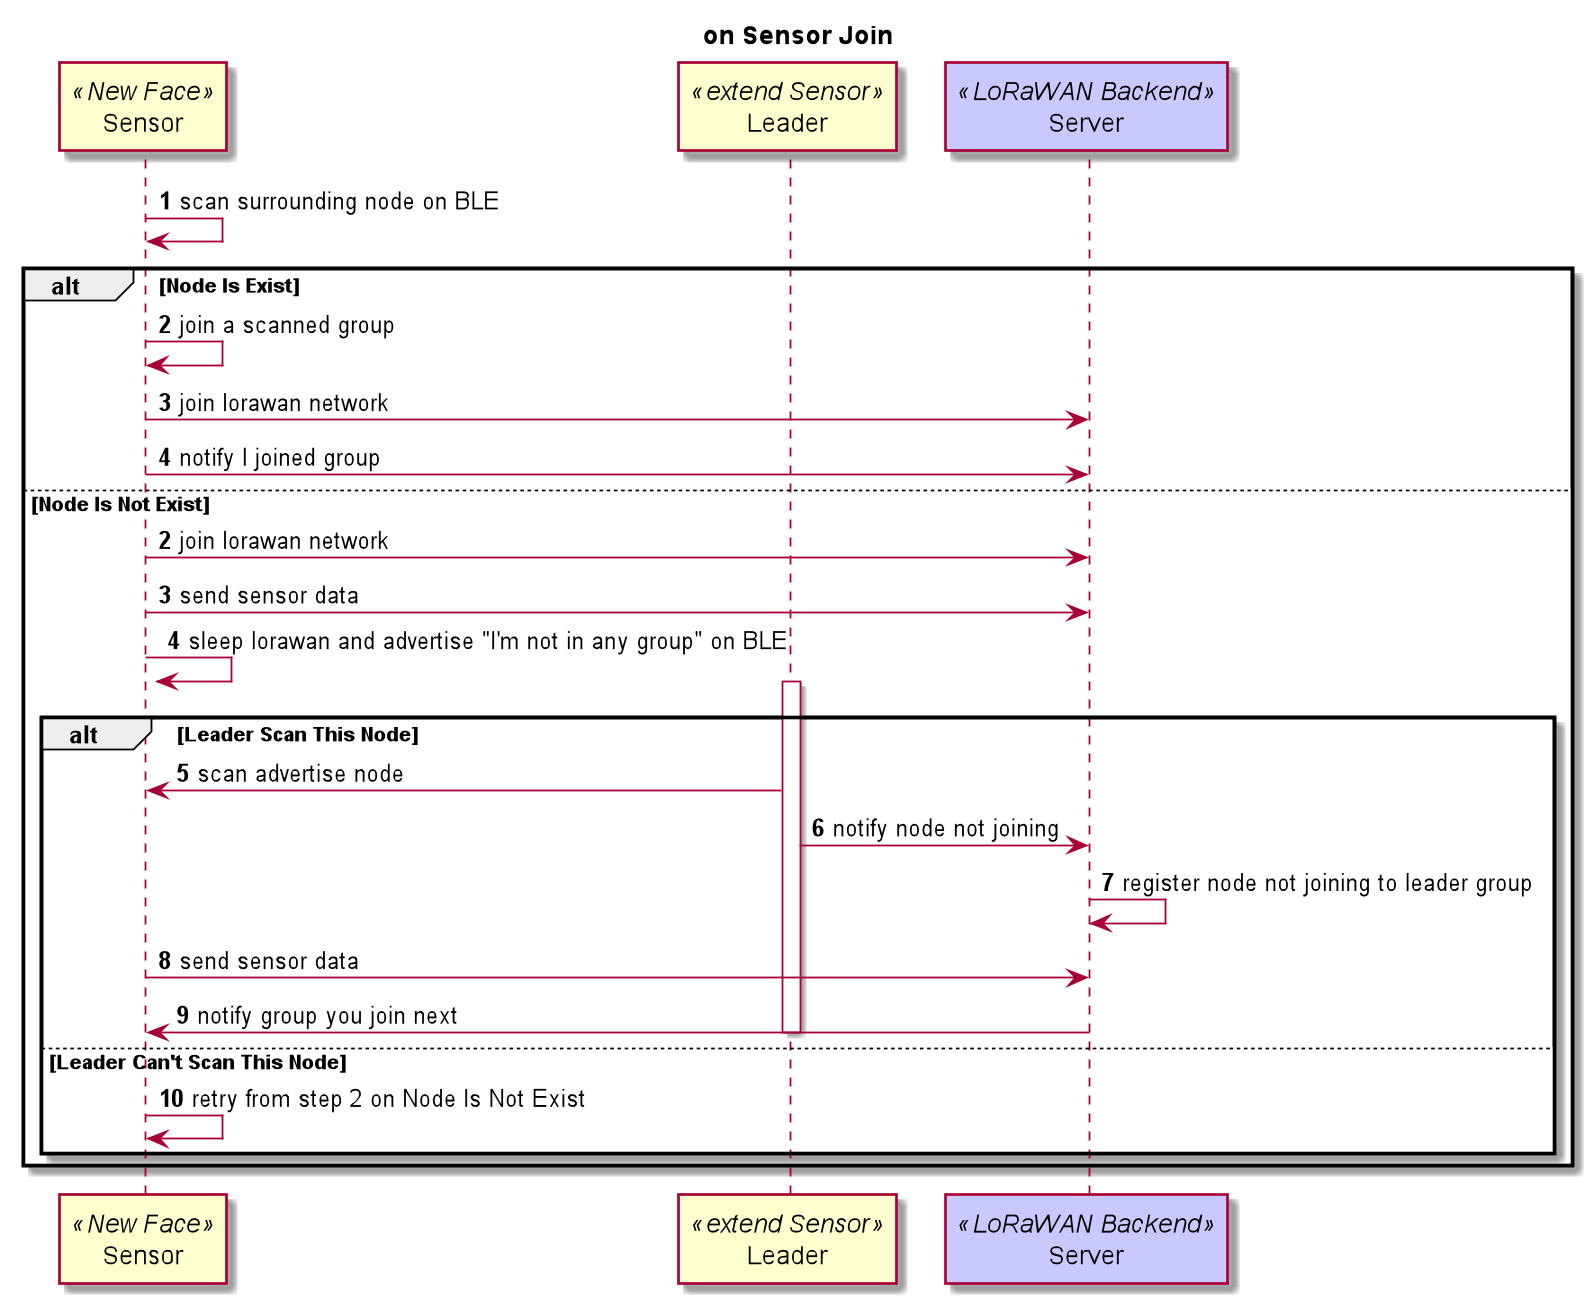
\includegraphics[width=14cm]{figures/グループ化_ネットワーク参加時.png}
    \caption{ネットワーク参加時の振る舞い}
    \label{fig:group_on_join}
    \end{center}
\end{figure}


\begin{figure}[]
    \begin{center}
    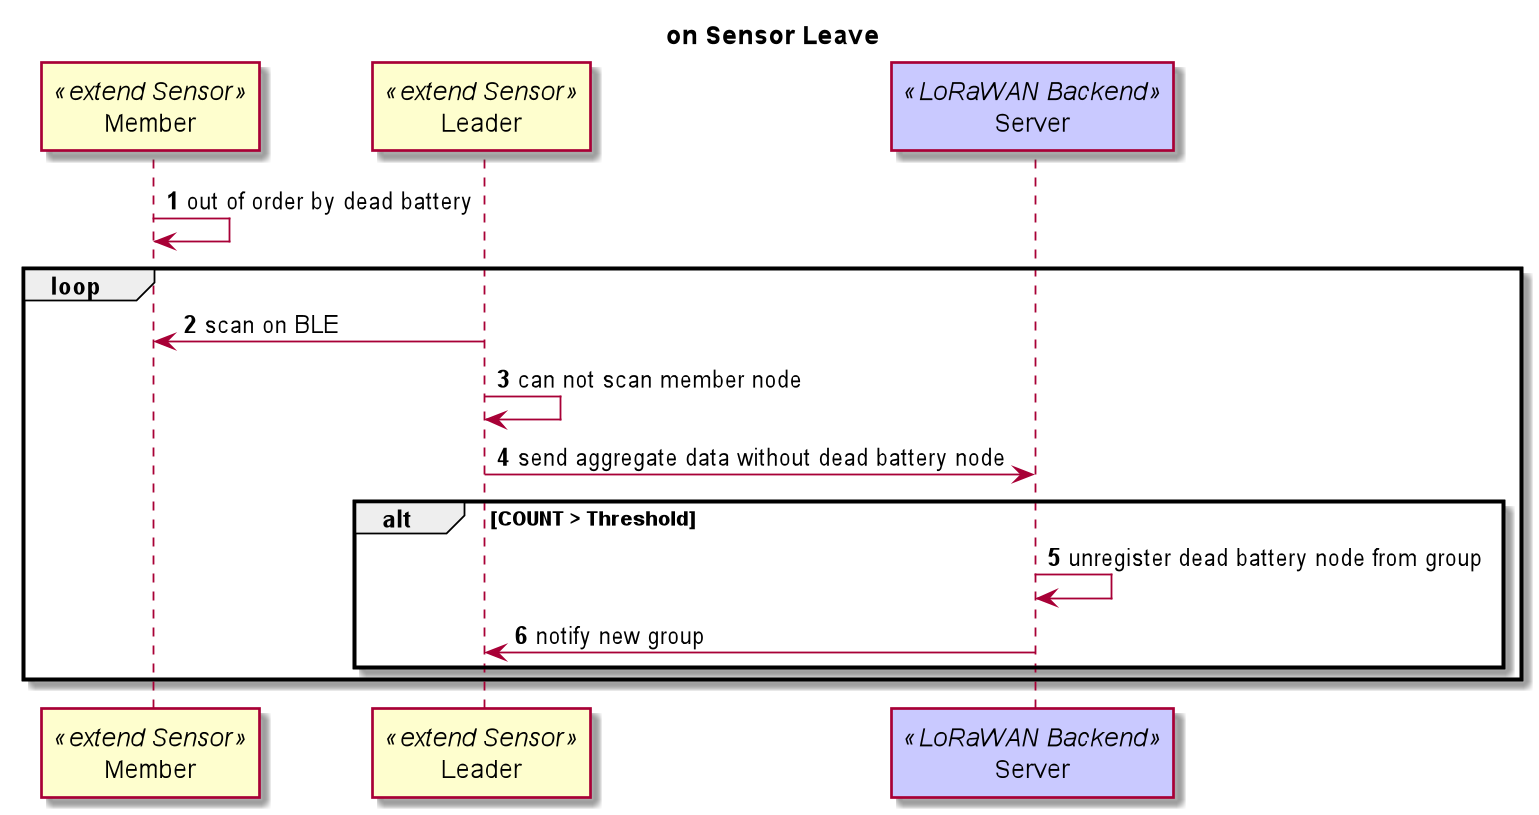
\includegraphics[width=14cm]{figures/グループ化_ネットワーク離脱時.png}
    \caption{ネットワーク離脱時の振る舞い}
    \label{fig:group_on_leave}
    \end{center}
\end{figure}